\FloatBarrier
\clearpage
\section{Fresh paired experiment: visuals and decisions}\label{sec:fresh}
The follow-up experiment re-ran both pretrained models on a new frozen snapshot:
999 closed BTCUSDT hourly candles ending at opening time 25 October 2026 00:00
UTC. It matches the requested dashboard settings: $L=128$, $H=12$, $S=20$,
and seed 42. Sixty non-overlapping label windows are split into 20 earlier
calibration origins with labels spanning 24 September 18:00 through 4 October
17:00 UTC, and 40 later test origins with labels spanning 4 October 18:00
through 24 October 17:00 UTC. The test
contains 480 horizon observations, but only 40 chronological origins. The
snapshot, model revisions, origins, source hashes, economic rules, and plotted
values are identified in \code{evidence/visual-evaluation-summary.json} and
the figure receipts~\cite{fresh}. No fresh fine-tuning or orders were performed.

\subsection{Both models must beat a useful baseline}
Chronos-2's native \code{predictions} column is its q50 median, despite the
library's compatibility name for a mean~\cite{chronosmedian}. The primary
location comparison therefore scores both medians; Kronos's sample mean is
also reported. Kronos receives OHLCVA while this Chronos adapter receives close
and past volume. This compares the implemented pipelines rather than isolating
architecture with identical input channels.

\begin{table}[htbp]\centering\small
% Generated from evidence/visual-evaluation-summary.json.
\begin{tabular}{lrrr}
\toprule
Point estimator & MAE & RMSE & Terminal dir. \\
\midrule
Persistence & 459.08 & 658.08 & 0.00\% \\
Kronos sample mean & 460.13 & 646.90 & 52.50\% \\
Kronos median & 467.02 & 653.50 & 55.00\% \\
Chronos-2 median & 499.24 & 700.86 & 50.00\% \\
\bottomrule
\end{tabular}

\caption{Fresh 40-origin held-out point scores. MAE/RMSE are USDT; terminal
direction has 40 observations. Persistence predicts the separate flat class.}
\label{tab:fresh-point}
\end{table}
Kronos median MAE is \FreshKMedianMAE{}, below Chronos's \FreshCMedianMAE{},
but persistence is lower still at \FreshBaselineMAE{} USDT. Kronos sample mean
MAE, \FreshKMeanMAE{}, also fails to beat persistence, although its RMSE is
slightly lower. An exploratory paired moving-block bootstrap of origin-level
MAE differences (four-origin blocks, 2,000 draws, seed 42) gives Kronos minus
Chronos \FreshBootstrapDifference{} USDT with a 95\% percentile interval
$[\FreshBootstrapLow{},\FreshBootstrapHigh{}]$. It crosses zero and is
conditional on this asset, period, and sampling run; it does not establish a
persistent model ranking.

\begin{table}[htbp]\centering\small
% Generated from evidence/visual-evaluation-summary.json.
\begin{tabular}{llrrr}
\toprule
Model & Interval & Coverage & Width & Pinball \\
\midrule
Kronos & Raw & 38.33\% & 478.60 & 186.37 \\
Kronos & Expanded & 73.75\% & 1200.93 & 159.35 \\
Chronos-2 & Raw & 72.50\% & 1384.79 & 169.57 \\
Chronos-2 & Expanded & 76.04\% & 1481.92 & 169.57 \\
\bottomrule
\end{tabular}

\caption{Fresh test uncertainty, 480 origin--horizon closes. Width and pinball
loss are USDT. Each model has its own frozen earlier-label expansion.}
\label{tab:fresh-interval}
\end{table}
Expansion improves coverage, but neither model reaches nominal 80\% on this
test. Kronos's raw intervals are especially narrow for the realized moves.
Its sample-vote Brier score is 0.30073, worse than the separate neutral
0.5-probability benchmark's 0.25. Interval expansion does not calibrate votes.
Across 61 native Kronos forecasts, 67 of 14,640 decoded candles violate an OHLC
bound, with no nonpositive OHLC or negative volume/amount values. Violations
are exposed without repair; the latest forecast has zero such violations.

\FloatBarrier
\subsection{What the latest forecast chart says}
\begin{figure}[htbp]\centering
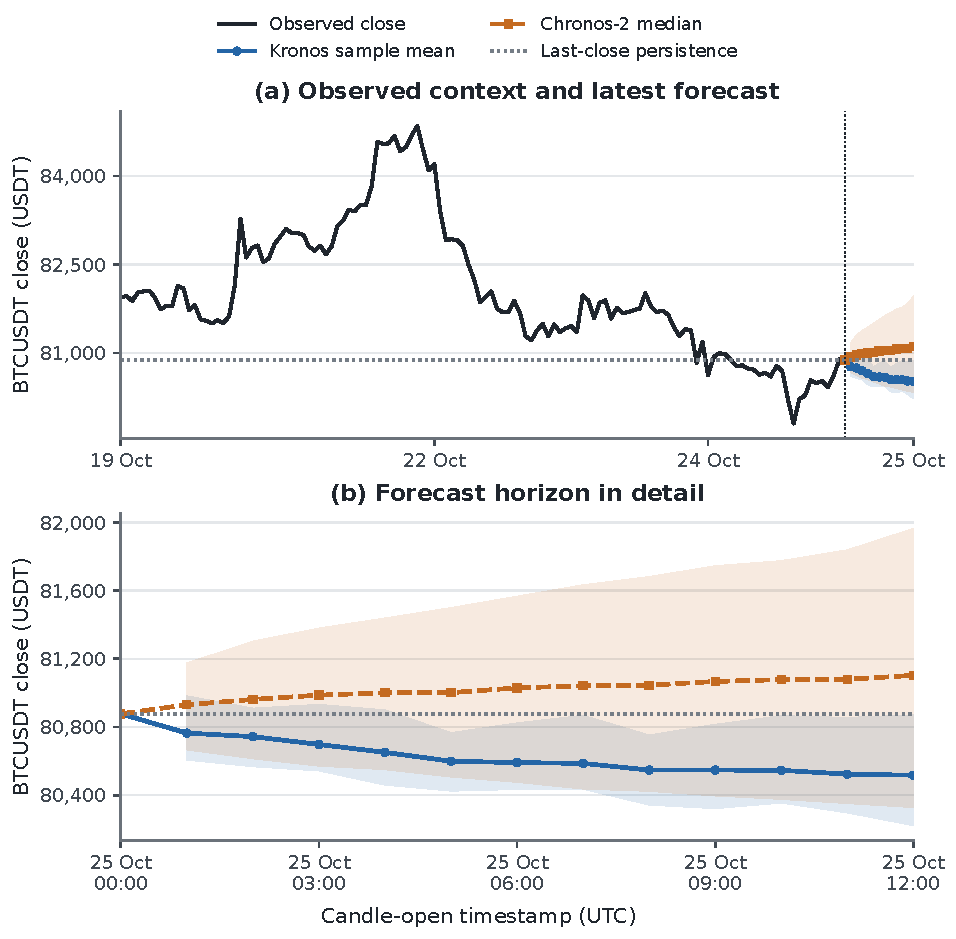
\includegraphics[width=\linewidth,height=.66\textheight,keepaspectratio]{figures/latest_forecast.pdf}
\caption{Fresh observed context and latest forecast detail. Blue is the Kronos
sample mean, orange the Chronos median, shading their raw q10--q90 intervals,
and the dotted horizontal line last-close persistence. Candle labels are opening
times; each plotted close occurs one hour later. Future actuals are not shown.}
\label{fig:latest-fresh}
\end{figure}
Figure~\ref{fig:latest-fresh} separates a point estimate from the spread of
possible outcomes. At issue time 25 October 01:13 UTC (08:13 in Ho Chi Minh
City), the last observed close is 80,877.25 USDT. The native point forecasts
disagree. Kronos has 2 of 20 terminal paths above that anchor; the 10\% vote
is not a 90\% reliable sell probability.

\begin{table}[htbp]\centering\small
% Generated from evidence/visual-evaluation-summary.json.
\begin{tabular}{lrrl}
\toprule
Model point & 12h return & Raw range (USDT) & Cost rule \\
\midrule
Kronos mean & -0.445\% & 80221.17--80871.20 & FLAT \\
Chronos median & +0.279\% & 80327.58--81965.02 & FLAT \\
\bottomrule
\end{tabular}

\caption{Latest 12-hour paper signal. Ranges are raw terminal quantiles;
the cost filter uses the fixed \FreshThreshold{} break-even threshold.}
\end{table}
Under the declared spot LONG/FLAT policy, Kronos's negative \FreshKReturn{}
does not select a new LONG. Chronos's positive \FreshCReturn{} is smaller than
assumed roundtrip friction, so its cost-aware rule also selects FLAT. The
agreement-and-cost policy consequently says \textbf{FLAT: no new buy under this
rule}. FLAT denotes cash or the policy's scheduled exit, not a short sale or a
recommendation to liquidate an existing portfolio. The expanded Kronos terminal
range (79,807.80--81,284.57) crosses the anchor, allowing a move against its point
forecast. That anchor is a closed-candle price, not a current executable quote.

\FloatBarrier
\subsection{What the walk-forward charts reveal}
\begin{figure}[htbp]\centering
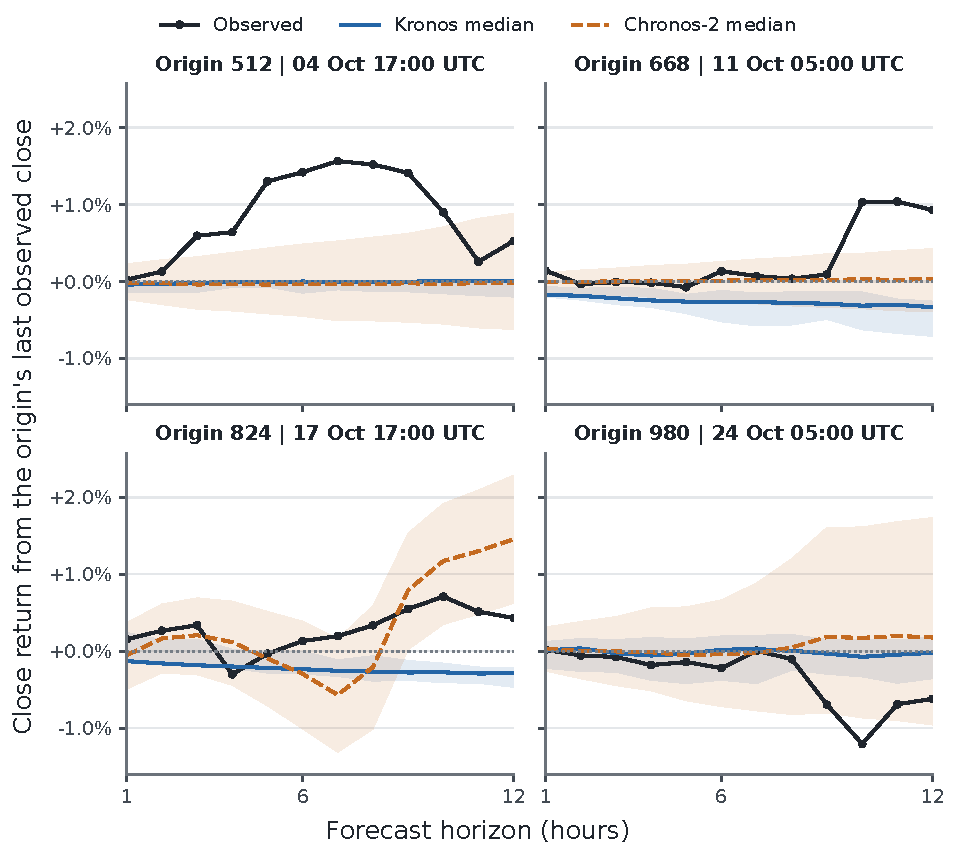
\includegraphics[width=\linewidth,height=.64\textheight,keepaspectratio]{figures/heldout_forecasts.pdf}
\caption{Four predetermined chronological test origins: first, two evenly spaced
interior origins, and last (512, 668, 824, 980). Both models predict the same
closes. Lines use medians, bands raw q10--q90, and returns use each origin's
observed anchor. Shared scales permit comparison; panels were not chosen for
model success.}
\label{fig:heldout-fresh}
\end{figure}
The black realized path in Figure~\ref{fig:heldout-fresh} often leaves Kronos's
narrow raw band. The orange band accommodates more outcomes partly because
it is wider. An individual plausible curve cannot identify the better trading
rule. Figure~\ref{fig:errors-fresh} includes all 40 test origins and uncertainty
by horizon, avoiding a conclusion based only on these four illustrations.

\begin{figure}[htbp]\centering
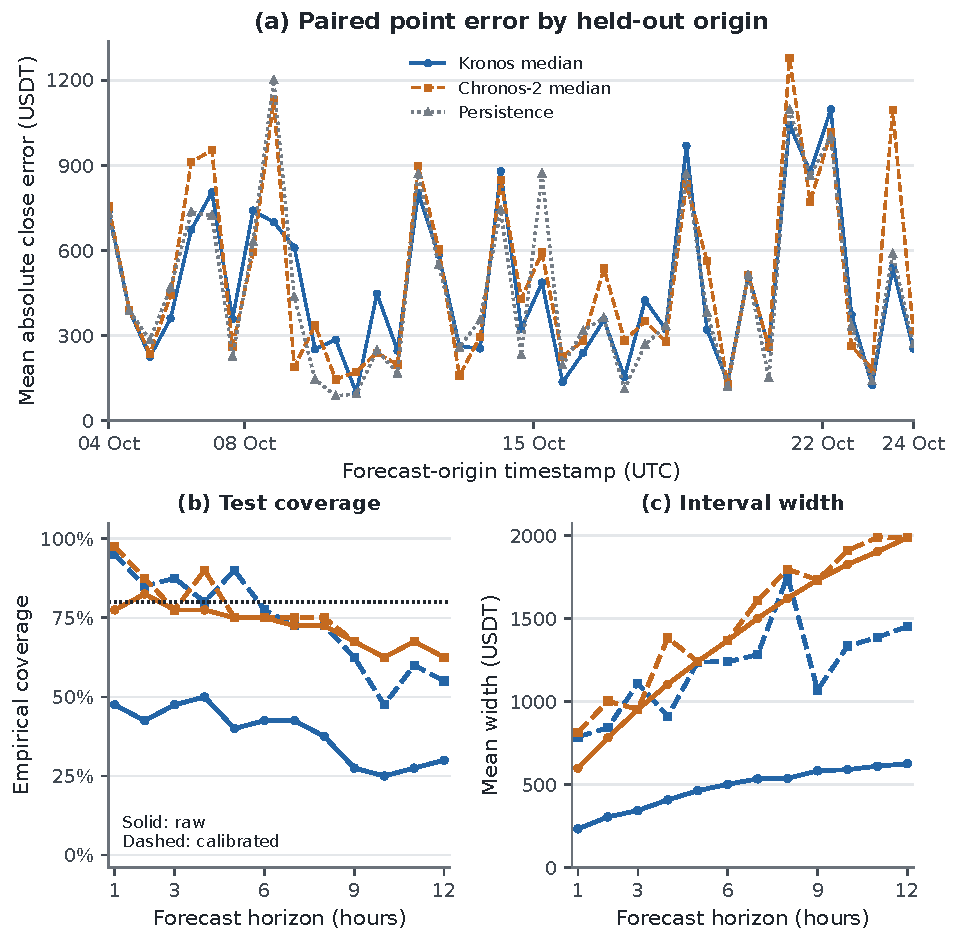
\includegraphics[width=\linewidth,height=.66\textheight,keepaspectratio]{figures/paired_errors_calibration.pdf}
\caption{All 40 test origins and all 12 horizons. Upper: median-based MAE
against persistence at matching origins. Lower: raw and expanded coverage and
width; each coverage point uses 40 closes. The 80\% guide is nominal. Wider
intervals can raise coverage while offering less precise predictions.}
\label{fig:errors-fresh}
\end{figure}
The error advantage changes across origins, and coverage deteriorates at some
horizons. This supports monitoring error and calibration through time. Neither
the bootstrap interval nor aggregate persistence MAE establishes a uniformly
superior model. No future coverage guarantee follows from either plot.

\FloatBarrier
\subsection{Which rule made money, and which won more trades?}
Rules were declared before inspecting scored results. Positive-return rules
buy when the native point return exceeds zero. Cost-filtered rules instead
require return above
\[
 b=\frac{(1+s)(1+f)}{(1-s)(1-f)}-1=0.003004505\ldots,
 \qquad f=0.001,\quad s=0.0005.
\]
The agreement rule requires both models to clear $b$. Historical 12-hour momentum,
cash, and one continuous buy-and-hold roundtrip provide references. No threshold,
ensemble weight, or selected strategy is fitted on test outcomes. The threshold
uses last close; the next open and actual fill are unknown at decision time.

\begin{table}[htbp]\centering\small
% Generated from evidence/visual-evaluation-summary.json.
\begin{tabular}{lrrrrr}
\toprule
Rule & Trades & Win rate & Net & Max DD & Costs \\
\midrule
Kronos positive & 13 & 23.08\% & -8.34\% & 9.17\% & 3.74\% \\
Chronos positive & 26 & 34.62\% & -12.28\% & 13.20\% & 7.27\% \\
Kronos cost filter & 5 & 40.00\% & -1.42\% & 4.12\% & 1.47\% \\
Chronos cost filter & 7 & 57.14\% & -2.20\% & 3.51\% & 2.07\% \\
Agreement + cost & 2 & 50.00\% & 0.44\% & 2.29\% & 0.60\% \\
12h momentum & 19 & 15.79\% & -14.42\% & 15.61\% & 5.38\% \\
Cash & 0 & -- & 0.00\% & 0.00\% & 0.00\% \\
Buy and hold & 1 & 0.00\% & -6.19\% & 7.90\% & 0.29\% \\
\bottomrule
\end{tabular}

\caption{Eight fixed paper rules on the same test period. Net return and
cumulative fee-plus-slippage costs are percentages of initial equity; sampled
drawdown is the percentage decline from running peak equity. Win rate counts strictly profitable executed trades; cash has no trade
win rate. Buy-and-hold is one continuous trade, not 40 paid roundtrips.}
\label{tab:fresh-strategies}
\end{table}
Agreement-and-cost has the highest observed net return, \FreshConsensusNet{},
but only two trades, 50\% trade win rate, and 2.29\% maximum sampled drawdown.
That is too little trading evidence to establish dominance, especially after
comparing eight candidates. Cash earns 0\% with no modeled drawdown. Both naive
positive-return rules lose money.

\textbf{Winning more trades is not the same as making more money.} The Chronos
cost filter wins 57.1\% of seven trades yet loses 2.20\% net. Agreement wins
50\% of two trades yet ends slightly positive. Payoff size, losses, turnover,
and costs determine the difference. Forecast directional accuracy cannot settle
it. Hypothetical backtests and realized investing are different evidence, and
costs and selected periods change a performance claim~\cite{performance}.

\begin{figure}[htbp]\centering
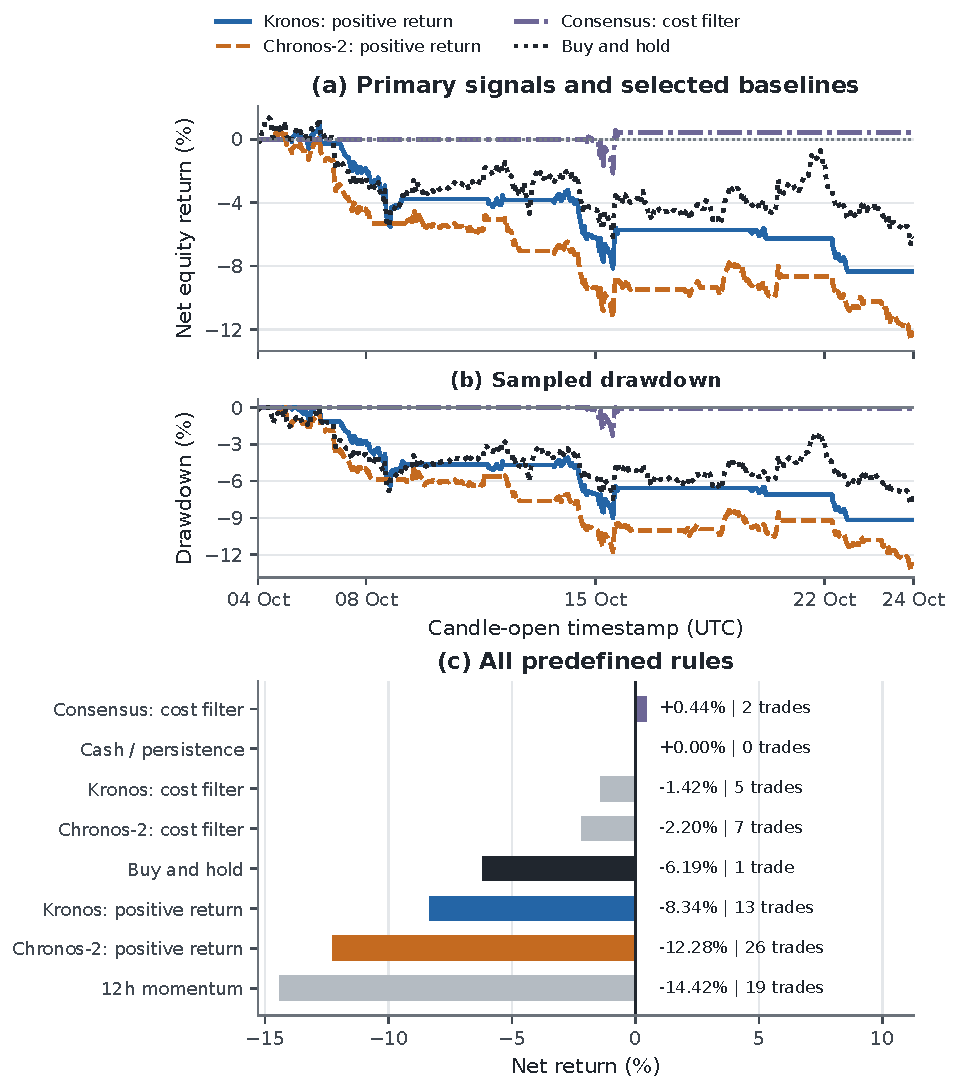
\includegraphics[width=\linewidth,height=.76\textheight,keepaspectratio]{figures/strategy_equity.pdf}
\caption{Net paper equity, sampled drawdown, and every fixed rule's net return
and trade count. Curves highlight model-positive rules, consensus, buy-and-hold,
and the best observed rule if different; the lower panel retains every candidate.
Costs are included. Drawdown uses ledger marks, not intrabar lows. There is no
annualized or general winning-strategy claim.}
\label{fig:equity-fresh}
\end{figure}
The evidence supports continued paper monitoring of the cost gate, with cash
as an explicit alternative, rather than an automatically deployed winner. No
short strategy was tested. Next-open paper execution assumes zero inference
latency, which the latest run's issue time does not achieve. Actual spreads,
liquidity, costs, and position risk can further change returns.

\FloatBarrier
\subsection{Actual dashboard captures}
These browser screenshots show the new real exports loaded through the actual
saved-result interface. This preserves the 20-calibration/40-test run; the
interactive evaluation button uses its smaller eight-window default. Each PNG
has a receipt linking it to its source JSON hash. No credentials were loaded.
Chart labels were enlarged for print; data and summary values are unchanged.

\begin{figure}[!htbp]\centering
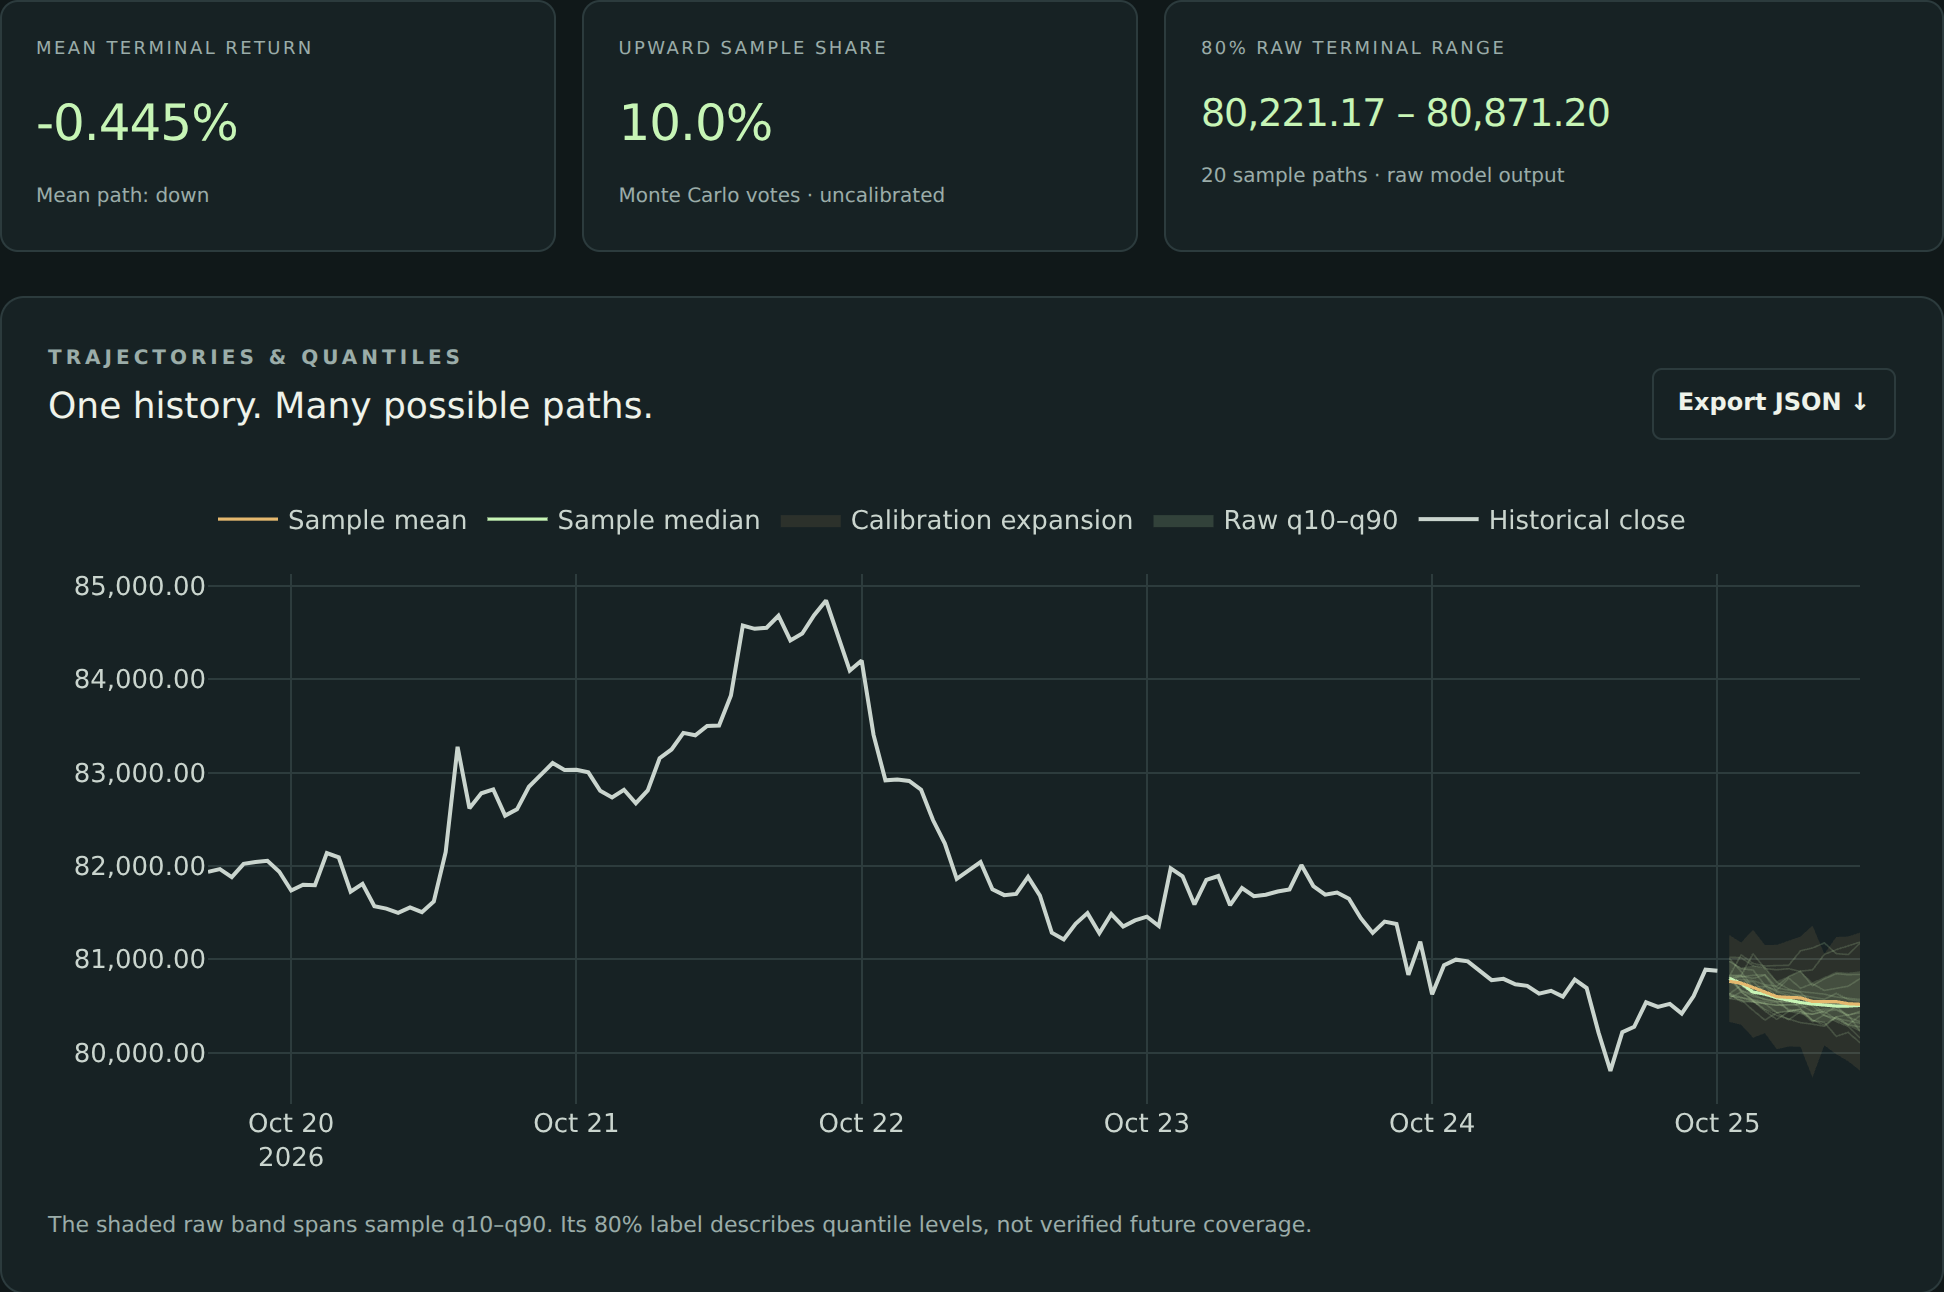
\includegraphics[width=\linewidth,height=.40\textheight,keepaspectratio]{figures/forecast-dashboard.png}
\par\medskip
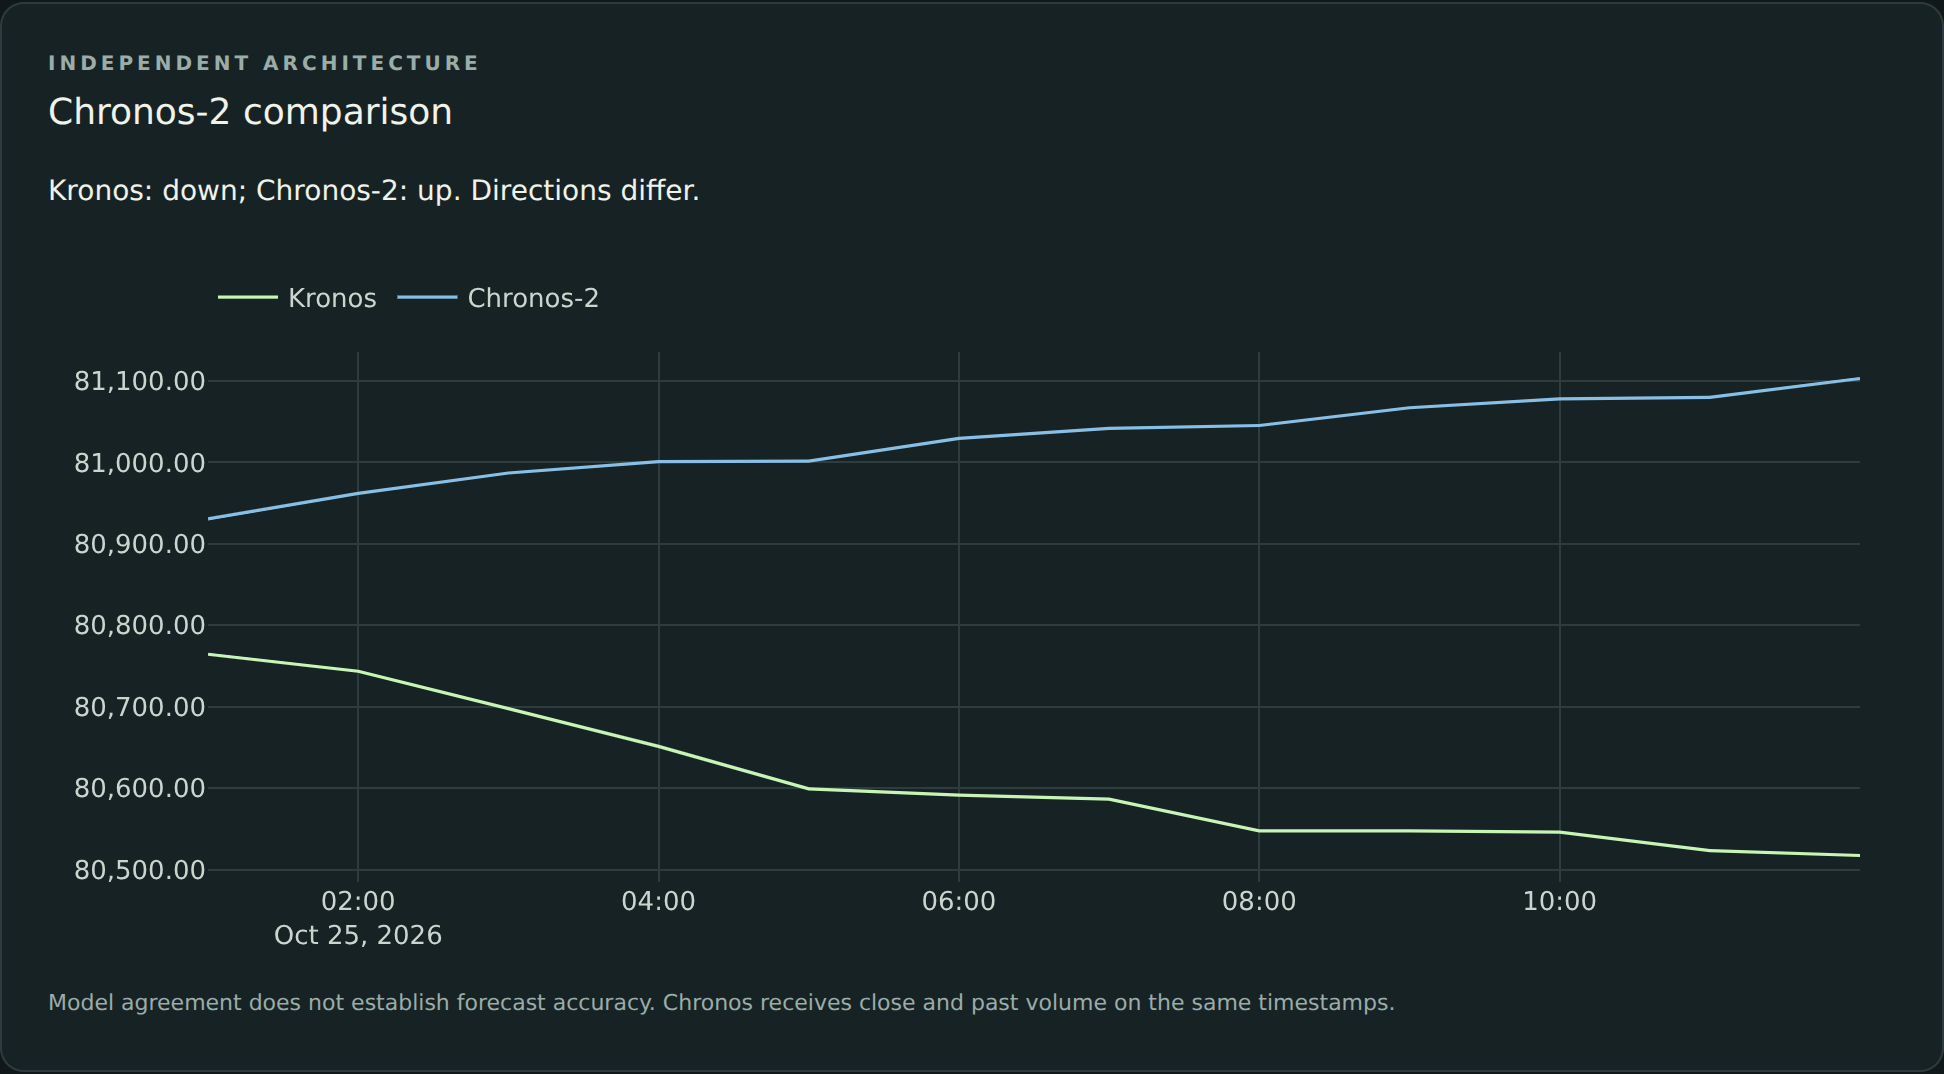
\includegraphics[width=\linewidth,height=.32\textheight,keepaspectratio]{figures/comparison-dashboard.png}
\caption{Actual dashboard captures. Upper: forecast fan, negative sample-mean
return, 10\% upward sample share, and raw terminal quantiles; these do not
establish a sell probability. Lower: Kronos sample mean trends down and Chronos
median trends up, but Chronos's gain still fails the cost gate. Both panels are
prospective, without realized future labels.}
\end{figure}
\begin{figure}[htbp]\centering
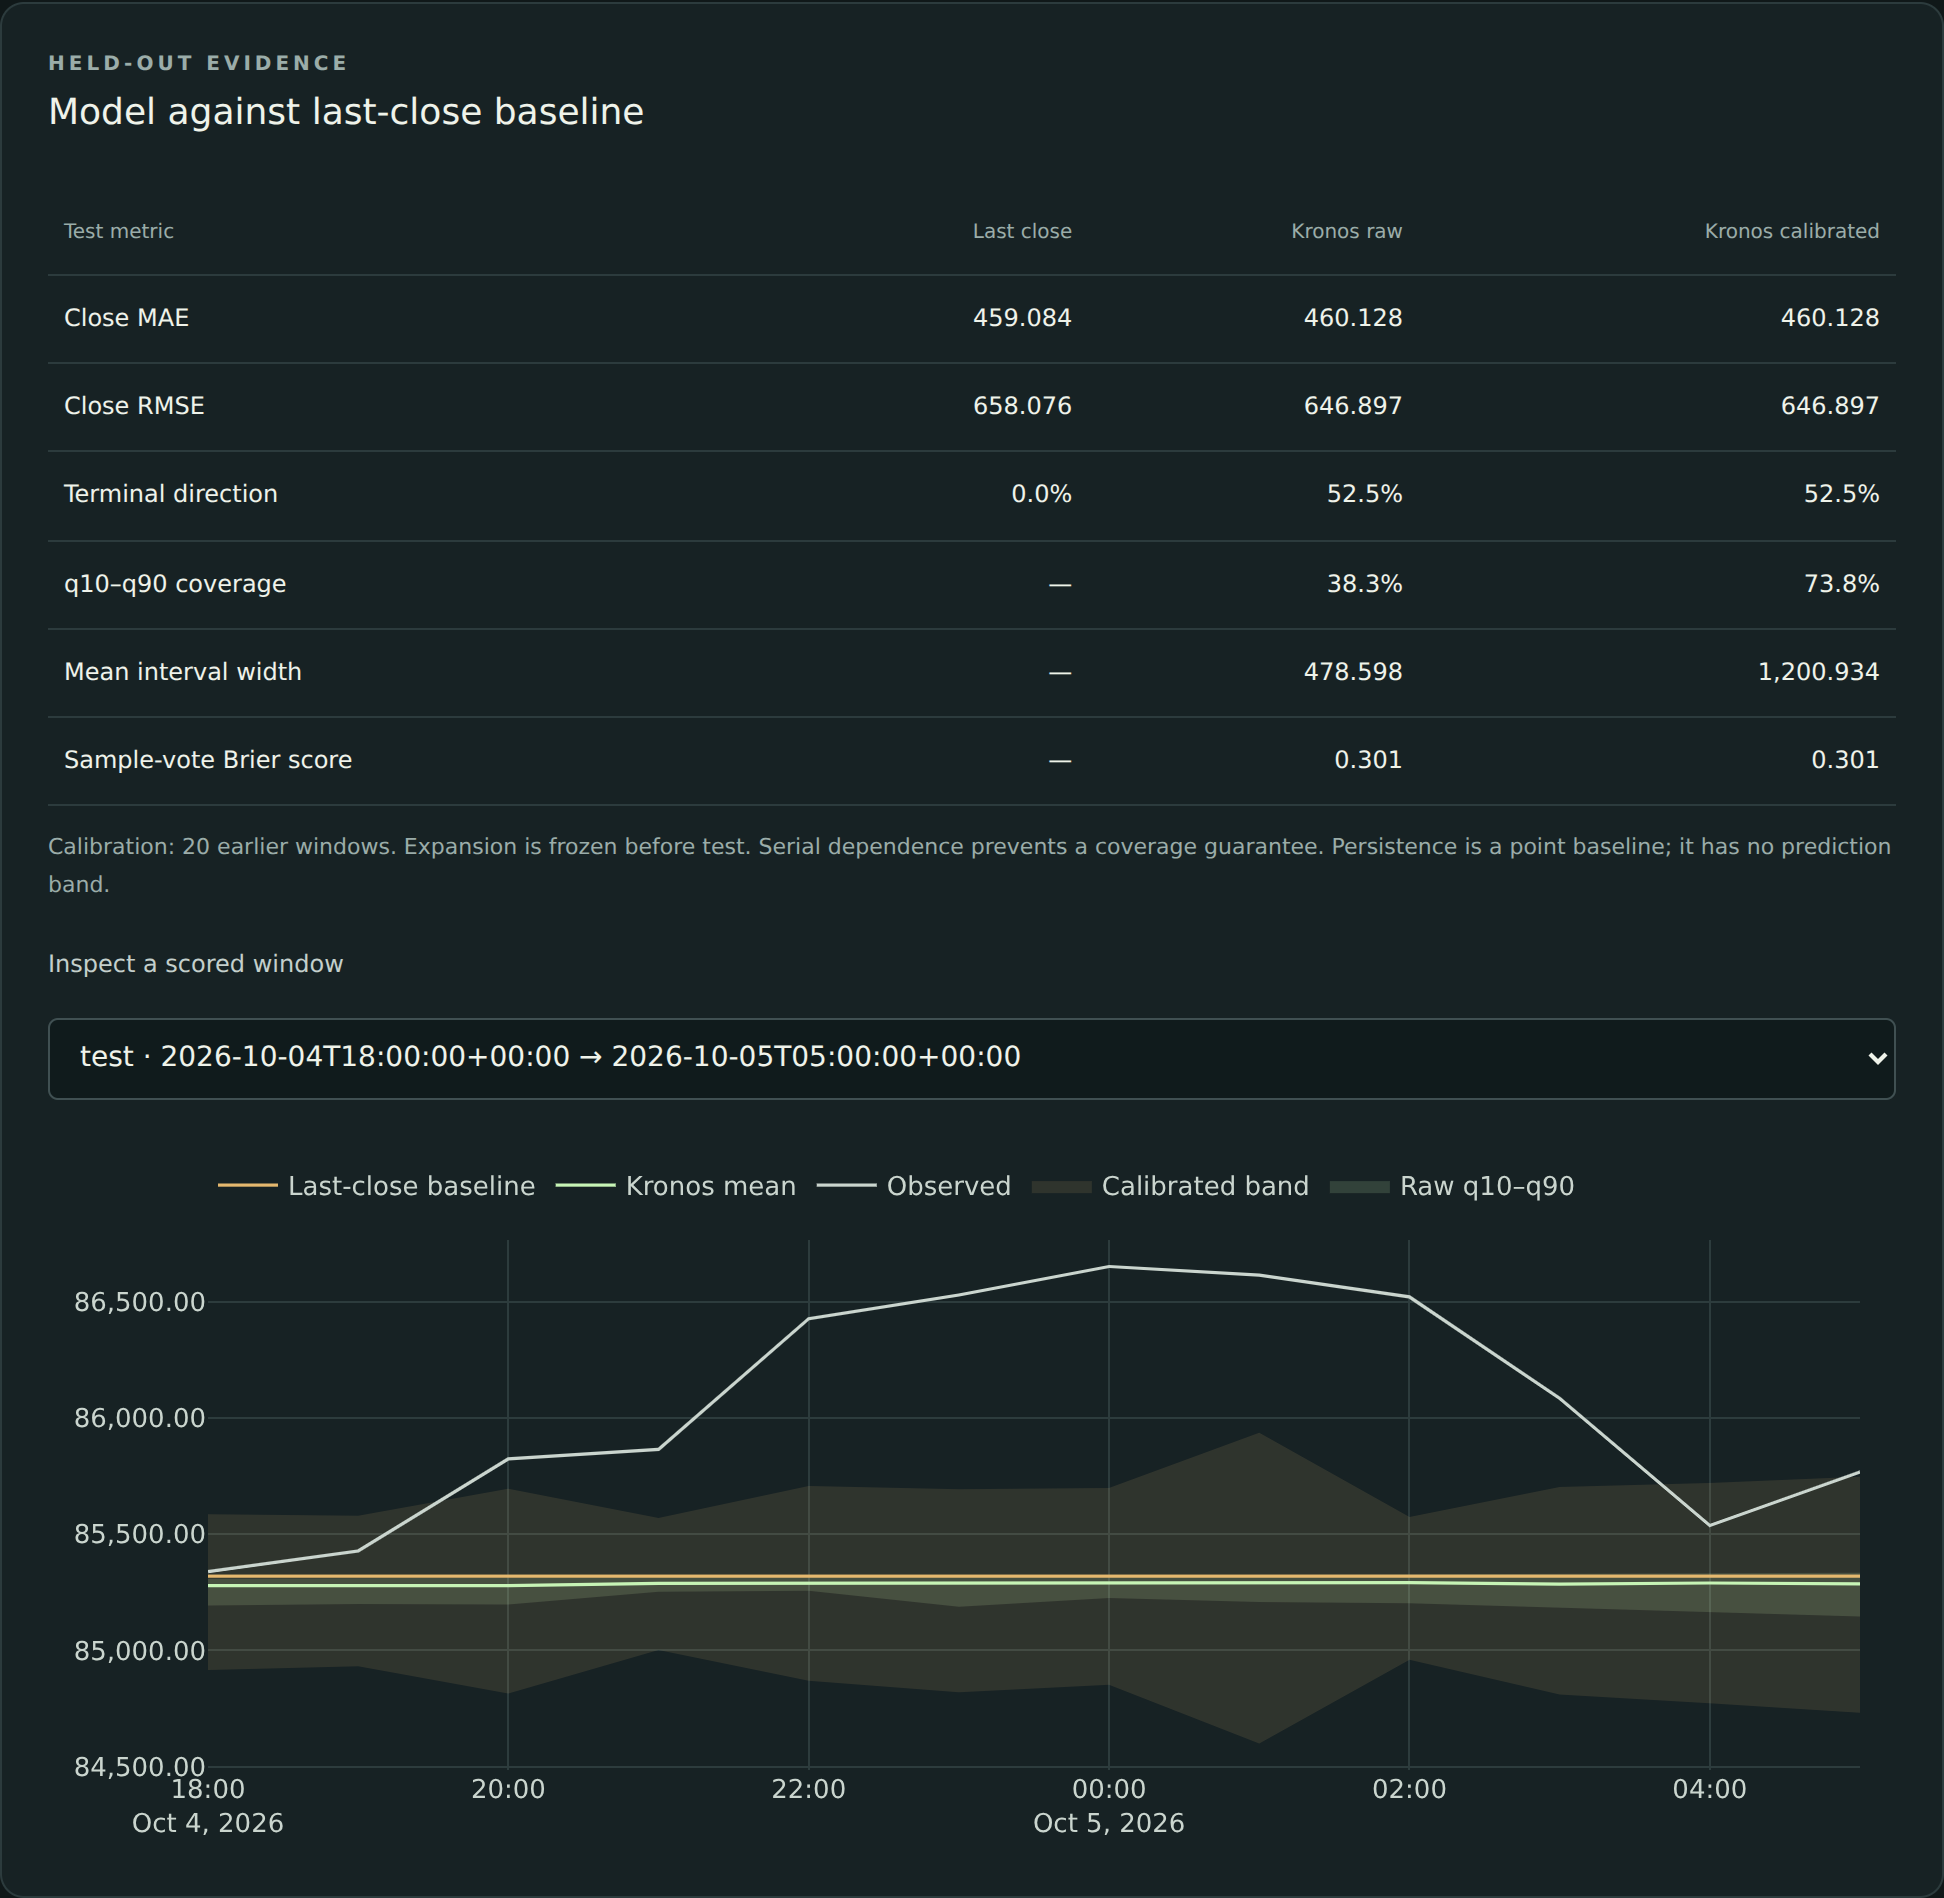
\includegraphics[width=\linewidth,height=.65\textheight,keepaspectratio]{figures/evaluation-dashboard.png}
\caption{Actual walk-forward dashboard: all 40 test-origin aggregate metrics
and first test window, origin 512. Its mean-based point score is
\FreshKMeanMAE{} versus persistence \FreshBaselineMAE{} USDT. The aligned
comparison in Table~\ref{tab:fresh-point} also supplies both medians.}
\end{figure}
\FloatBarrier
